\newcommand\chapternumber{1}
\documentclass[12pt,a4paper]{article}
\usepackage{fullpage}
\usepackage[top=2cm, bottom=4.5cm, left=2.5cm, right=2.5cm]{geometry}
\usepackage{amsmath,amsthm,amsfonts,amssymb,amscd}
\usepackage{lastpage}
% \usepackage{enumitem}
\usepackage{fancyhdr}
\usepackage{mathrsfs}
\usepackage{xcolor}
\usepackage{graphicx}
\usepackage{listings}
\usepackage{hyperref}
\usepackage{tikz}
\usetikzlibrary{shapes,backgrounds}
\usepackage[utf8]{inputenc}
\usepackage[ruled, vlined]{algorithm2e}
% \usepackage{apacite}
\usepackage{csquotes}

% Edit these as appropriate
\newcommand\course{Data Science II}
\newcommand\NetID{sliu1@uvm.edu}
\newcommand\Author{Sida Liu}
\pagestyle{fancyplain}
\headheight 35pt
\lhead{\NetID\\\Author}
\chead{\textbf{\Large \pagetitle }}
\rhead{\course \\ \today}
\lfoot{}
\cfoot{}
\rfoot{\small\thepage}
\headsep 1.5em

\setlength{\parskip}{\baselineskip}%
\setlength{\parindent}{0pt}%

\newenvironment{list_abc}
{ \begin{enumerate}[label=(\alph*)] }
    { \end{enumerate} }

\newenvironment{list_iv}
{ \begin{enumerate}[label=\roman*.] }
    { \end{enumerate} }

\hypersetup{
  colorlinks=true,
  linkcolor=blue,
  filecolor=magenta,
  urlcolor=cyan,
}

\usepackage[overload]{empheq}
\usepackage{tikz}
\usetikzlibrary{bayesnet}
\usetikzlibrary{arrows}

\usepackage{xparse}
\NewDocumentCommand\Cycle{O{} m m m O{} m}{%
% [opt arg cycle]{Node}{Angle}{Node size}[opt arg arch node]{cycle size}
\draw[#1](#2.{#3+asin(#6/(#4*1.41))}) arc (180+#3-45:180+#3-45-270:#6/2) #5;
}

% no color for hyperlinks
\usepackage{hyperref}
\hypersetup{
  colorlinks=true, 
  citecolor=blue, 
  linkcolor=blue, 
  urlcolor=blue
}

\usepackage{enumerate}
\usepackage{float}

\begin{document}

\section*{What is Data Science?}

``Data Science" is a new term which has started to gain public attention in recent years.

\begin{figure}[h]
    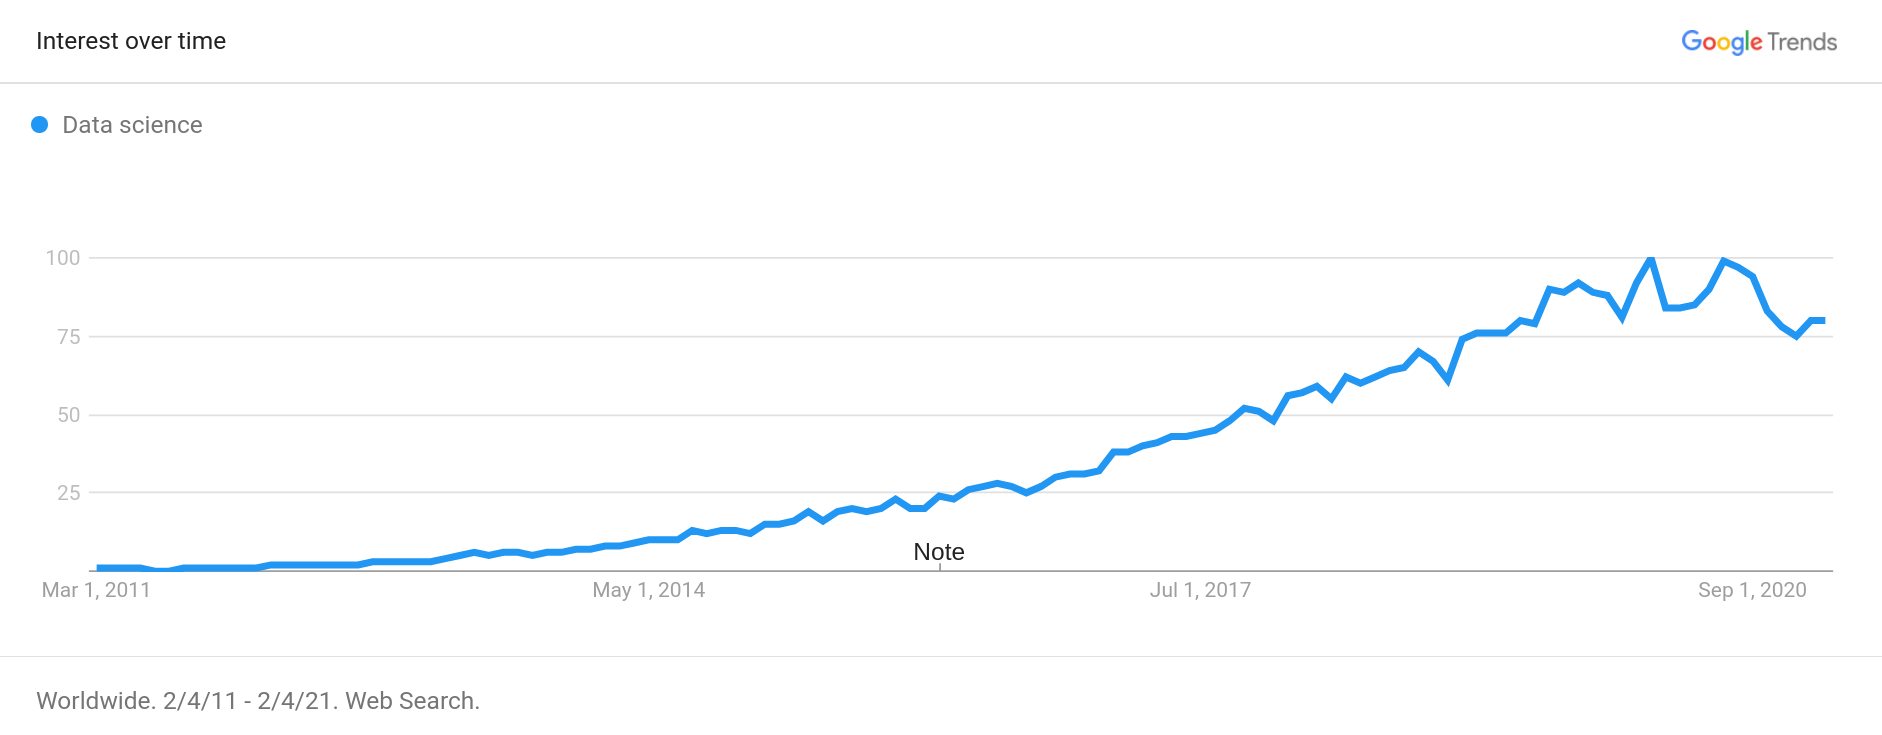
\includegraphics[width=\textwidth]{images/google_trend_1.png}
    \caption{From Google Trends \cite{Google_Trends}}
\end{figure}


However, as a field of study, ``Data Science'' is still very young, and
the popularity of this term is relatively small compared to those well-established disciplines.
This is why there is still no convention on what it is, and we still need to discuss the necessity of this discipline.

\begin{figure}[h]
    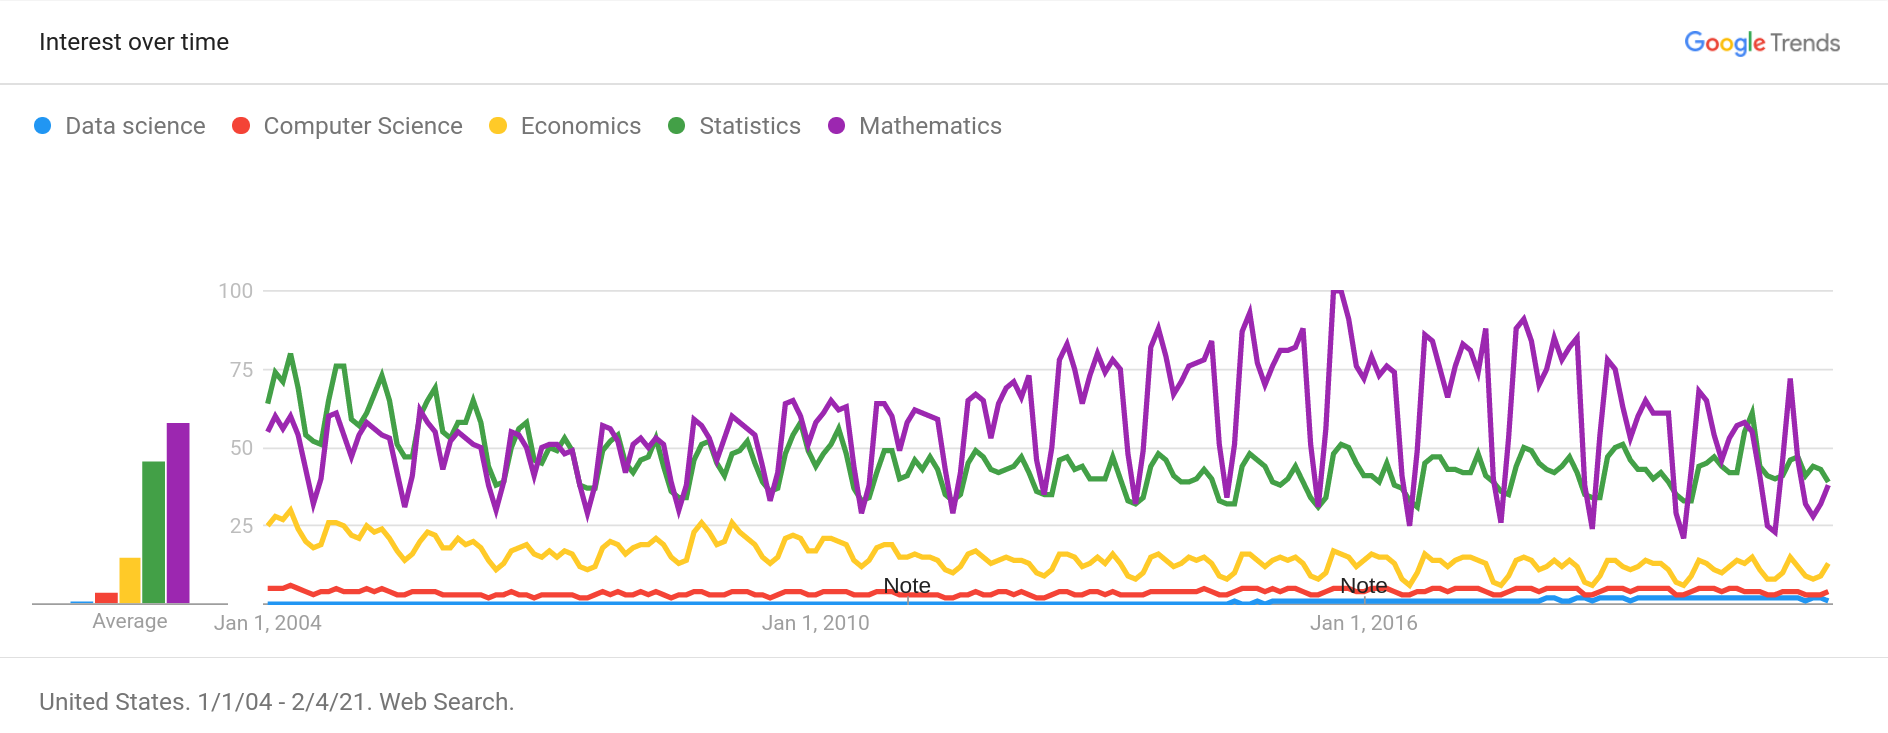
\includegraphics[width=\textwidth]{images/google_trends.png}
    \caption{From Google Trends \cite{Google_Trends}}
\end{figure}

\newpage
The ``Data Science'' revolution started almost back in 1962, when Tukey called for a reformation of statistics to meet the needs of increasingly complicated data processing in science \cite{tukey_future_1962}.
In the following decades, many other scholars followed this idea \cite{donoho_50_2017}.
However, the interest was bounded within the academia.
Partially because the academia was much more data-intensive than the industry back then.

Recently, the rise of internet and especially the smart phones, makes the whole society much data-intensive than the past.
Before the internet, maybe a normal person was only represented by several bytes, such as in a survey or a Yellow Pages, but now anyone with a smart phone can easily consume or produce gigabytes of data.
Thus one can build companies to provide data that people want to consume, or to mine values from the data that people produced.
We can see, not only the academia cares about data, the industry also cares about data.
And we entered the ``Big Data'' era.

So, in general, this term ``Data Science'' can be two things: a discipline in the academia, or a business in the industry.
In this assignment, we only discuss the former one.

First, let's discuss why data science should exist in the first place.
Imagine that when people carry out scientific research, they will do experiments which produce data, and those data, after appropriate processes, become evidence that support the hypotheses behind those experiments.

If an experiment only produces, say, 100 numbers, there is even no need for a computer, it is completely possible to do statistics by hand.
And it's true that people did scientific research way before computers were invented.
However, if an experiment produces thousands and thousands of numbers, it is obvious that a computer can facilitate the process.
When an experiment produces gigabytes or even terabytes of data, the process of handling these data becomes a hard problem, we need algorithms to accelerate the process and make good use of resources, otherwise we might never be able to wait until the evidence finally comes out.
When an experiment produces gigabytes or terabytes of data with thousands and thousands of different formats, it's not just as easy as applying one sophisticated algorithm, but it needs data science now. 
So, the most important mission of data science is to handle the ``Data Deluge" \cite{hey_data_2003}, making use of them but not being drained by them.

With this in mind, let's compare data science to other disciplines and the intersections of these disciplines.

\subsection*{Computer Science v.s. Data Science}

Data science needs tools and skills from computer science.
Without those tools, one cannot handle data at such a large scale.
However, computer science is not just a discipline that invents tools for handling large-scale data.
What data science actually uses is produced in a subfield of computer science.

On the other hand, the tools and skills cannot represent the whole spirit of data science, they just help solving problems.
Data science uses those tools but not equal to those tools.

\subsection*{Statistics v.s. Data Science}

Statistics works well in guiding the experiment design and the inference of the data.
However, when there is ``Data Deluge" \cite{hey_data_2003}, the traditional statistics, which works in theory, might not work anymore simply because the computational resource is not enough.
Data science is rooted from statistics, but it aims to handle large-scale problems. 

There might be a phase transition from statistics to data science, since the scale of data increases dramatically.
For example, the emphasis of statistics is inference of the unknown parameters in the model, but when the number of those parameters becomes too large, they cannot be easily understood by humans anymore, so the emphasis of data science might shift to prediction, which is much easier to understand in terms of accuracy.

\subsection*{Mathematics v.s. Data Science}

Mathematics is not as close as previous two disciplines.
Mathematics develops a perfect world with well-defined rules.
Some of the rules happen to be aligned with the real world, and people can use those rules to summarize phenomena or do predictions.
However, these applications are by-products of mathematics, and mathematics is not aiming to solely serve for this purpose. 
Data science utilize tools from mathematics to achieve its goal when necessary.

\subsection*{Economics v.s. Data Science}

Economics, as a discipline, is quite different from data science.
Economics is a social science which care about the production, distribution, and consumption of goods and services \cite{webster_economics}.
It can utilize data science to do advanced research, but data science is not developed for economics.
For data science, it might be pretty much the same when helping economics and genomics.

(When we think data science as an industry, which is outside the scope of this article, it might relate more with economics. The economics in the big-data era might have some unique characteristics.)

\subsection*{Data Science as the intersection of Statistics and Computer Science}

In 2017, data science was described as the intersection of statistics and computer science \cite{blei_science_2017}.

\begin{displayquote}
The foundational goals of data science rely on statistical thinking...
Statistical thinking provides methods to answer scientific questions with data.
Computational thinking focuses on the algorithmic implementation of those methods, and it provides a way to understand and compare their computational footprints.
\end{displayquote}

We can view data science as the offspring of those two disciplines.
Just like any offsprings in nature, data science share similarity with its parents, but it developed its own unique characteristics.

Data scientists need to be the data stewards, develop algorithms to analyze and adapt different file formats \cite{mattmann_vision_2013}, use any tools that is available to integrate data systems so that the data can produce valuable knowledge for high-level decision making.

And like any parents in nature, they might have other offsprings as well. 
For example, when we brought statistics and computer science together, deep learning also emerged, and people can use it to control robots.

\subsection*{Other intersections}

As we discussed, to data science, mathematics and economics are not as close as computer science and statistics.
So we briefly discuss the other intersections:

\subsubsection*{Computer Science + Mathematics}

Computer science itself is an offspring of mathematics.
Now computer science has been well developed, and has the ability to help its parent mathematics to do more interesting research.

\subsubsection*{Computer Science + Economic}

Economics can study the impact of computer science, and computer science can help economics study other things.

\subsubsection*{Statistics + Mathematic}

Statistics constantly uses tools from mathematics, so I guess this intersection is part of statistics itself.

\subsubsection*{Statistics + Economic}

Economics constantly uses tools from statistics, so I guess this intersection is part of economics itself.

\subsubsection*{Mathematics + Economic}

Based on the last two outcomes above, I guess this intersection is also part of economics itself.

\newpage
\subsection*{Why should I want to spend money on a data scientist?}

In the context of academia, we should fund data scientists because they can facilitate large experiments.
Without them, it is hard for normal scientists to even properly store the data produced by large experiments, not even to mention to process them and make the best use of the data.

In the context of industry, if we are business owners, we should spend money on data scientists because they make the companies more competitive in the big-data era.

Computer engineers could follow the specifications and make good software, but they usually do not understand what the business goals are.
On the other hand, people in a high position usually don't have the ability or time to access raw data without help.

But data scientists can bridge the high-level decision making group directly to the raw data.
So if there are many values in the data, data scientists are the best choice to turn them into profit.

\bibliographystyle{plain}
\bibliography{reference.bib}

\end{document}